\documentclass[10pt,a4paper,titlepage]{article}
\usepackage[utf8]{inputenc}
\usepackage{amsmath}
\usepackage{amsfonts}
\usepackage{amssymb}
\usepackage{amsthm}
\usepackage{biblatex}
\usepackage{mathtools}
\usepackage{csquotes}
\usepackage[bottom]{footmisc}
\usepackage{pgfplots}
\usepackage{listings}
\usepackage{graphicx}
\usepackage{chngcntr}
\usepackage[hypertexnames=false]{hyperref}

\graphicspath{ {./img/} }

%\usepackage{parskip}
\pgfplotsset{compat=1.16}
\usetikzlibrary{patterns}



% Python Code style
% Default fixed font does not support bold face
\DeclareFixedFont{\ttb}{T1}{txtt}{bx}{n}{8} % for bold
\DeclareFixedFont{\ttm}{T1}{txtt}{m}{n}{8}  % for normal

% Custom colors
\usepackage{color}
\definecolor{deepblue}{rgb}{0,0,0.5}
\definecolor{deepred}{rgb}{0.6,0,0}
\definecolor{deepgreen}{rgb}{0,0.5,0}

% Python style for highlighting
\newcommand\pythonstyle{\lstset{
language=Python,
basicstyle=\footnotesize,
otherkeywords={self, None, True, False},             % Add keywords here
breaklines=true,
keywordstyle=\ttb\color{deepblue},
emph={MyClass,__init__},          % Custom highlighting
emphstyle=\ttb\color{deepred},    % Custom highlighting style
stringstyle=\color{deepgreen},
frame=tb,                         % Any extra options here
showstringspaces=false,            % 
captionpos=b,
numbers=left,
numbersep=5pt
}}


% Python environment
\lstnewenvironment{python}[1][]
{
\pythonstyle
\lstset{#1}
}
{}

% Python for external files
\newcommand\pythonexternal[2][]{{
\pythonstyle
\lstinputlisting[#1]{#2}}}

% Python for inline
\newcommand\pythoninline[1]{{\pythonstyle\lstinline!#1!}}

\addbibresource{references.bib}
%\bibliography{references}

\author{Felix Fritz}
\title{The Bondareva-Shapley Theorem}

\theoremstyle{plain}
\newtheorem{thm}{Theorem}[section] % reset theorem numbering for each chapter

\theoremstyle{definition}
\newtheorem{definition}[thm]{Definition} % definition numbers are dependent on theorem numbers
\newtheorem{example}[thm]{Example} % same for example numbers
\newtheorem{lemma}[thm]{Lemma}

\newcount\colveccount
\newcommand*\colvec[1]{
        \global\colveccount#1
        \begin{pmatrix}
        \colvecnext
}
\def\colvecnext#1{
        #1
        \global\advance\colveccount-1
        \ifnum\colveccount>0
                \\
                \expandafter\colvecnext
        \else
                \end{pmatrix}
        \fi
}

\begin{document}
\counterwithin{lstlisting}{section}
\maketitle

\tableofcontents
\pagebreak


\section{Cooperative Games and the Core}
Before diving into the concept of balanced collections, balanced games and the Bondareva-Shapley Theorem, I want to establish a basic understanding of cooperative games, imputations and the core, mainly as it is described in Robert P. Gilles book \cite{gilles}, pp. 12--13, 18--20 and 29--35.

\begin{definition}
    The pair $(N, v)$ is a \textit{cooperative game} if $N$ is a finite player set and $v: 2^N \rightarrow \mathbb{R}$ is a characteristic function that assigns to every coalition $S \subseteq N$ an attainable payoff $v(S)$ such that $v(\emptyset) = 0$.
    
    For every player set $N$ we denote by $\mathcal{G}^N$ the class of all characteristic functions on $N$.
\end{definition}
Simply put, in a cooperative game collective payoff values are defined for every possible coalition between players. A coalition with no players leads to a payoff of zero.

Suppose for a given cooperative game all players form a grand coalition generating a total payoff of $v(N)$. The ways in which this collective wealth can be distributed is described by a vector $x \in \mathbb{R}^N$, each element $x_i$ indicating what player $i \in N$ would receive.
If this vector fulfills the requirement needed for efficiency and individual rationality, then it is described as an \textit{imputation}.

\begin{definition}
    An \textit{imputation} in the cooperative game $v \in \mathcal{G}^N$ is a vector $x = (x_1, ..., x_n) \in \mathbb{R}^N$ satisfying
    \[
        \begin{aligned}
            &x(N) = v(N) && \quad \text{(Efficiency)}\footnotemark\\
            &x_i \geq v(i)\text{ for every player } i \in N && \quad \text{(Individual rationality)\footnotemark}
        \end{aligned}
    \]
    \footnotetext[1]{For a given vector $x \in \mathbb{R}^N$ and a coalition $S \subseteq N$, $x(S)$ refers to the sum of elements $x_i$ for each player $i \in S$: $x(S) = \sum_{i \in S}x_i$}
    \footnotetext{Formally we would need curly braces around $i$ in the payoff function $v$ $\rightarrow v(\{i\})$. Because it is obvious that $v(i)$ indicates the payoff for a coalition containing the single player $i$, I will omit the braces.}
    The set of all vectors satisfying the efficiency and individual rationality constraint is the \textit{imputation set}.
    \begin{equation}\label{eq:imputation}
        I(N, v) \coloneqq \{x \in \mathbb{R}^N \mid x(N) = v(N),\quad x_i \geq v(i) \quad \forall i \in N\}
    \end{equation}
\end{definition}

With the imputation set, each player is ensured to receive his individual value at minimum.

If each possible coalition $S \subseteq N$ is taken into account to verify that the value from an imputation $x(S) = \sum_{i \in S}x_i \geq v(S)$, then the imputation is \textit{coalitionally rational}.

\begin{definition}\label{def:core}
    A collection of coalitionally rational imputations is the \textit{core} of a cooperative game.
    \begin{equation}\label{eq:core}
        \mathcal{C}(N, v) \coloneqq \{x \in I(N, v) \mid x(S) \geq v(S)\quad \forall S \subseteq N\}
    \end{equation}
\end{definition}


%%% CHAPTER 2 - Bondareva-Shapley Theorem %%%


\pagebreak
\section{Bondareva-Shapley Theorem}
In the following chapter I will discuss the properties of cooperative games with a nonempty core and introduce the notion of balancedness, which leads me to the Bondareva-Shapley Theorem.

\subsection{Nonempty Cores}
This section's focus will be on some of the properties that need to apply for a cooperative game to have at least one imputation that is coalitionally rational, or in other words has a nonempty core.

\begin{example}
    A cooperative game with $N = 2$ players has the following attainable payoffs: $v(\emptyset) = 0, v(1) = v(2) = 2, v(1, 2) = 3$.

    Determining if a core exists in such a situation may be trivial to solve, but with only two players this gives us the opportunity to plot a graph and visualize the solution concept.
    
    Because this is only a two-player game, there are no coalitions other than the grand coalition. This means that every imputation is automatically inside the core.
    
    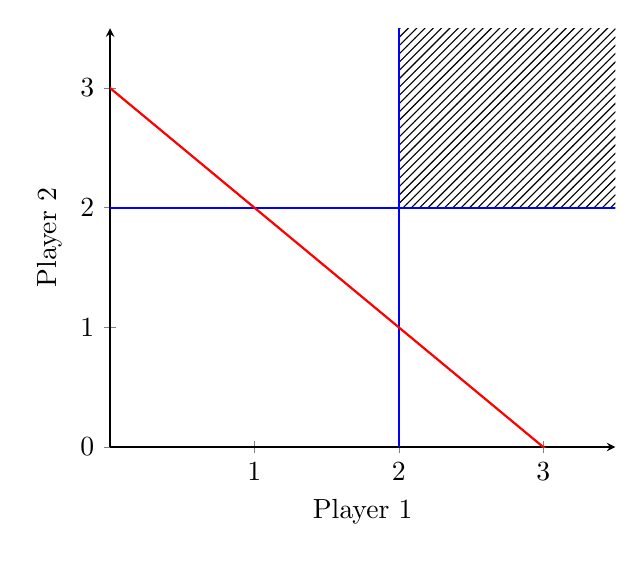
\begin{tikzpicture}
        
        \begin{axis}[no marks,
            axis lines = left,
            xlabel = {Player 1},
            ylabel = {Player 2},
            xmin = 0, xmax = 3.5,
            ymin = 0, ymax = 3.5,
            xtick={1,2,3},
            width=8cm
        ]
            
            %what player 1 wants
            \filldraw [draw=none,pattern=north east lines] (2, 2) rectangle (3.5, 3.5);
            \addplot [blue, thick]{2};
            \addplot [blue, thick] coordinates {(2,0)(2,3.5)};
            

            %efficient payoff function
            \addplot [color=red, thick]{-x+3};
        \end{axis}
        % \filldraw [draw=none,pattern=north east lines] (3.6, 3) rectangle (6.5, 5.5);
            
    \end{tikzpicture}
\end{example}

Because the grand coalition generates a value of 3, an efficient vector $x(N) = x_1 + x_2 = 3$. From this we can derive the function $f(x_2) = 3 - x_1$, which is shown in the graph by the red diagonal line.

The horizontal and vertical lines could be described as the \enquote{individually rational} plots, indicating that because of $v(1) = v(2) = 2$ each player in a coalition would like to receive a payoff of 2 at minimum. This means that the smallest attained payoff that would cause the players to form a grand coalition is at the point where the two lines intersect, which is at $(2, 2)$ generating a payoff of 4. From this point, every vector to the upper right would be seen as profitable by the players.

Because none of the actual vectors on $f(x_2)$ cross that region, the cooperative game has an empty core. For a game with two players to have a nonempty core, $v(1, 2) \geq v(1) + v(2)$ must hold, which would be at $v(1, 2) \geq v(1) + v(2) = 2 + 2 = 4$ in the example's case.

Let's further investigate what properties have to apply for a three-player game to have a nonempty core.

\begin{example}\label{ex:findvalue}
    We are given a cooperative game with $N = 3$ players generating the following payoffs:

    \begin{tabular}{c | c c c c c c c}
        $S$ & $\emptyset$ & $\{1\}$ & $\{2\}$ & $\{3\}$ & $\{1, 2\}$ & $\{1, 3\}$ & $\{2, 3\}$\\
        \hline
        $v(S)$ & 0 & 2 & 2 & 1 & 3 & 4 & 6
    \end{tabular}

    What would the minimum payoff $v(1, 2, 3)$ have to be for the players to form a grand coalition?\vspace{10pt}

    To start off, consider the imputation set. For this it is only necessary to find a vector $x \in \mathbb{R}^3$ all vectors that fulfill $x_i \geq v(i)$.

    If every element of $x$ is set equal to the payoff of $v(i)$, this gives us a vector $x = (2, 2, 1)$. From this we derive that a payoff of $5$ would be sufficient for the game to have a nonempty imputation set.

    Clearly this is not the answer however, because players 2 and 3 would much rather get together than cooperate in a grand coalition. Thus, let's consider putting those two together and letting player 1 work on his own. This generates a collective value of $v(1) + v(2, 3) = 8$.

    To verify if this is correct, an imputation $x$ must be found so it is efficient ($x(N) = 8$) and individually and coalitionally rational. For now, I will choose $x = (2, 3, 3)$. This results in the following equations:

    \begin{alignat*}{7}
    x_1 &+ &x_2 &+ &x_3 &= 8 \quad&=&\quad 8 = v(1, 2, 3)\\
    x_1 &+ &x_2 &  &    &= 5 &\geq &\quad 3 = v(1, 2)\\
    x_1 &  &    &+ &x_3 &= 5 &\geq &\quad 4 = v(1, 3)\\
        &  &x_2 &+ &x_3 &= 6 &\geq &\quad 6 = v(2, 3)\\
    x_1 &  &    &  &    &= 2 &\geq &\quad 2 = v(1)\\
        &  &x_2 &  &    &= 3 &\geq &\quad 2 = v(2)\\
        &  &    &  &x_3 &= 3 &\geq &\quad 1 = v(3)
    \end{alignat*}

    This shows that a payoff of 8 would be enough for all three players to form a grand coalition.
\end{example}

However, looking for an arbitrary imputation that \textit{might} be in the core set may not always be as trivial as it was for our example, especially if such problems should be solved computationally. Furthermore finding a payoff vector should be irrelevant if we're only interested in the total attained payoff.

To find a \textit{\enquote{value-based}} approach, I will make use of M. Maschler, E. Solan and S. Zamir's book \enquote{Game Theory} \cite{maschler} (p. 691 ff).

Because the payoff vector is efficient ($x(N) = v(N)$), the inequalities from example \ref{ex:findvalue} can be transformed as follows.

\begin{align}
    v(1) + v(2) + v(3) &\quad\leq\quad v(1, 2, 3)\\
    v(1, 2) + v(3) &\quad\leq\quad v(1, 2, 3)\\
    v(1, 3) + v(2) &\quad\leq\quad v(1, 2, 3)\\
    v(2, 3) + v(1) &\quad\leq\quad v(1, 2, 3)
\end{align}

This can be extended to a final inequality.

\begin{align*}
    (x_1+x_2)+(x_1+x_3)+(x_2+x_3) &\quad \geq \quad v(1, 2) + v(1, 3) + v(2, 3)\\[6pt]
    2*(x_1+x_2+x_3) &\quad \geq \quad v(1, 2) + v(1, 3) + v(2, 3)\\
    v(1, 2, 3) &\quad \geq \quad \frac{1}{2} v(1, 2) + \frac{1}{2} v(1, 3) + \frac{1}{2} v(2, 3)
\end{align*}

\addtocounter{thm}{-1}
\begin{example}\label{ex:valuebased}
    \textit{(continued)}

    Substituting the inequalities from previously where a vector $x$ was chosen with the inequalities just introduced, we get:
    \begin{align*}
        v(1, 2, 3) = 8\quad & \geq \quad 5 = v(1) + v(2) + v(3)\\
        v(1, 2, 3) = 8\quad & \geq \quad 4 = v(1, 2) + v(3)\\
        v(1, 2, 3) = 8\quad & \geq \quad 6 = v(1, 3) + v(2)\\
        v(1, 2, 3) = 8\quad & \geq \quad 8 = v(2, 3) + v(1)\\
        v(1, 2, 3) = 8\quad & \geq \quad 6.5 = 0.5*v(1, 2) + 0.5*v(1, 3) + 0.5*v(2, 3)
    \end{align*}
\end{example}

Those five inequalities are in fact already enough to prove that a payoff of 8 would make a grand coalition feasible. The reason for this will be discussed in chapter \ref{sec:bondareva}.



%%%% SUBSECTION 2.2 BALANCED COLLECTIONS %%%%

\subsection{Balanced Collections and Balancing Coefficients}
Each inequality in example \ref{ex:valuebased} \textit{(continued)} looks at the collective wealth of a \textit{balanced collection} of coalitions, each collection with its own set of \textit{balancing coefficients}. M. Maschler\cite{maschler} sums it up with the following table.\vspace{8pt}

\begin{tabular}{ | r l | c | }
    \multicolumn{2}{c}{Collection of coalitions} & \multicolumn{1}{c}{Coefficients}\\[2pt]
    \hline & & \\[-8pt]
    $\mathcal{B}_1 =$ & $\{\{1\}, \{2\}, \{3\}\}$ & $(1, 1, 1)$\\[2pt]
    $\mathcal{B}_2 =$ & $\{\{1, 2\}, \{3\}\}$ & $(1, 1)$\\[2pt]
    $\mathcal{B}_3 =$ & $\{\{1, 3\}, \{2\}\}$ & $(1, 1)$\\[2pt]
    $\mathcal{B}_4 =$ & $\{\{2, 3\}, \{1\}\}$ & $(1, 1)$\\[2pt]
    $\mathcal{B}_5 =$ & $\{\{1, 2\}, \{1, 3\}, \{2, 3\}\}$ & $(\frac{1}{2}, \frac{1}{2}, \frac{1}{2})$\\[2pt]
    \hline
\end{tabular}\vspace{8pt}

$\mathcal{B}_1$ through $\mathcal{B}_4$ are partitions of $N = \{1, 2, 3\}$ with each player appearing exactly once. This always gives us a set of coefficients where each element is 1. From this a \enquote{partition} rule can be deducted.

\begin{lemma}
    Let a cooperative game with $N$ players have a nonempty core. A partition is a collection of nonempty coalitions $\mathcal{B} = \{S_1, S_2, ..., S_k\}$ satisfying $S_i, S_j \subsetneq N, S_i \cap S_j = \emptyset$ iff\footnote{iff is shorthand for \enquote{if and only if}, also represented with the math symbol $\Leftrightarrow$} $i \neq j, S_1 \cup S_2 \cup ... \cup S_k = N$.

    Then for every partition $\mathcal{B}$ it must be the case that

    \begin{align}
        v(N) \geq \sum_{S \in \mathcal{B}} v(S)
    \end{align}
\end{lemma}

The goal now is to find a property that also includes the non-partition $\mathcal{B}_5$ from our three-player example. To do this I will use Maschler's\cite{maschler} definition on Index Matrices (p. 693).

\begin{definition}\label{def:incidencematrix}
    Let $\mathcal{B} = \{S_1, S_2, ..., S_k\}$ be a collection of nonempty coalitions.\footnote{Although collections are unordered, when defining $S_i$ and later on $\delta_i$ I will assume that index $i$ corresponds to the position at which this element was written. Eg. if $A = \{x, y, z\}$, $A_2$ refers to element $y$} The matrix $\mathcal{M}$ of $\mathcal{B}$ is the \textit{incidence matrix} with m rows (one for each player) and n columns (one for each coalition) with each index $x_{ij}$ at row $i = {1, ..., m}$ and column $j = {1, ..., n}$ defined as\vspace{-15pt}

    \begin{equation*}
        x_{ij} =
        \begin{cases}
            1 & \quad\text{if}\ i \in S_j\\
            0 & \quad\text{otherwise}
        \end{cases}
    \end{equation*}
\end{definition}

There is a slight difference to M. Maschler's\cite{maschler} definition in that the resulting matrices will be transposed (his columns represent players, not coalitions). This aligns more with Abhishek Gupta's\cite{youtube} definition (at 7:00) which will make later calculations a lot nicer visually.

\begin{example}\label{ex:indexmatrix}
    Given a cooperative game with $N = \{1, 2, 3\}$ and the collections of coalitions $\mathcal{B}_1 = \{\{1\}, \{2\}, \{3\}\}$, $\mathcal{B}_2 = \{\{1, 2\}, \{3\}\}$, $\mathcal{B}_5 = \{\{1, 2\}, \{1, 3\}, \{2, 3\}\}$, what is each corresponding incidence matrix?\vspace{8pt}

    $
    \bordermatrix{
    \mathcal{M}_1 & S_1 & S_2 & S_3 \cr
    1 & 1 & 0 & 0 \cr
    2 & 0 & 1 & 0 \cr
    3 & 0 & 0 & 1 \cr
    }
    $\hspace{35pt}$
    \bordermatrix{
    \mathcal{M}_2 & S_1 & S_2\cr
    1 & 1 & 0 \cr
    2 & 1 & 0 \cr
    3 & 0 & 1 \cr
    }
    $\hspace{35pt}$
    \bordermatrix{
    \mathcal{M}_5 & S_1 & S_2 & S_3 \cr
    1 & 1 & 1 & 0 \cr
    2 & 1 & 0 & 1 \cr
    3 & 0 & 1 & 1 \cr
    }
    $\vspace{8pt}
\end{example}

Interestingly, if each matrix is multiplied by its corresponding set of coefficients (here shown by the greek letter $\delta$), we get all-ones vectors.\vspace{-15pt}

\begin{alignat*}{4}
    \mathcal{M}_1 \delta_1 = &&\begin{pmatrix}
        1 & 0 & 0\\
        0 & 1 & 0\\
        0 & 0 & 1
    \end{pmatrix}&\colvec{3}{1}{1}{1} &= \colvec{3}{1}{1}{1}\\
%
    \mathcal{M}_2 \delta_2 = &&\begin{pmatrix}
        1 & 0\\
        1 & 0\\
        0 & 1
    \end{pmatrix}&\colvec{2}{1}{1} &= \colvec{3}{1}{1}{1}\\
%
    \mathcal{M}_5 \delta_5 = &&\begin{pmatrix}
        1 & 1 & 0\\
        1 & 0 & 1\\
        0 & 1 & 1
    \end{pmatrix}&\colvec{3}{1/2}{1/2}{1/2} &= \colvec{3}{1}{1}{1}
\end{alignat*}

If for a given collection of coalitions there exists a \textit{vector of positive coefficients} $\delta$ that after multiplying results in a all-ones vector, then the collection is called \textit{balanced}. Yakar Kannai\cite{kannai} (p. 359) defines it as follows.

\begin{definition}\label{def:balanced}
    The collection of coalitions $\mathcal{B} = \{S_1,..., S_k\}$  of $N$ is called \textit{balanced} if there exists a vector of positive numbers $\delta$ such that for every $i \in N$

    \begin{align}
        \sum_{i \in S_j} \delta_j = 1 && j = 1, ..., k
    \end{align}
    
    The numbers $\delta_1, ..., \delta_k$ are called \textit{balancing weights}. If $\delta$ contains at least one 0, then $\mathcal{B}$ is \textit{weakly balanced} and $\delta$ is called \textit{weakly balancing weights}.
\end{definition}

Martin Osborn\cite{osborne} (p. 262) offers an interpretation of balancing weights as \enquote{each player having one unit of time, which he\footnote{Despite the gender neutrality movement I will, for the sake of simplicity, view all players as males.} must distribute among all the coalitions of which he is a member.} For $\mathcal{B}_5$ in example \ref{ex:indexmatrix} this would mean for player 1 spending half of his time with player 2 and the other half with player 3. Since player 2 and 3 both have half their time taken up by player 1, they will also spend their last half together.

If $\mathcal{B}$ were unbalanced and some coefficients still had to be chosen, the resulting values from Definition \ref{def:balanced} for each player then could be interpreted as follows.\vspace{-15pt}

\begin{equation*}
    \sum_{i \in S_j} \delta_j
    \begin{cases}
        = 1\qquad \text{Player i is fully occupied}\\
        > 1\qquad \text{Player i is overworked}\\
        < 1\qquad \text{Player i does not have enough to do}
    \end{cases}
\end{equation*}

\begin{lemma}\label{lem:weaklybalanced}
    $\mathcal{B} = \{S_1,..., S_k\}$ is weakly balanced (but not limited to) if a group of coalitions $\mathcal{D} \subsetneq \mathcal{B}$ is balanced.

    Let $\delta$ and $\gamma$ be the balancing vectors for $\mathcal{B}$ and $\mathcal{D}$ respectively. The resulting weakly balancing weights $\delta_i$ for $i = 1, ..., k$ then are
    
    \begin{equation*}
        \delta_i =
        \begin{cases}
            \gamma_j & \quad\text{if there is one } j = 1, ..., |\mathcal{D}| \text{ such that }\mathcal{B}_i = \mathcal{D}_j\\
            0 & \quad\text{otherwise}
        \end{cases}
    \end{equation*}
\end{lemma}

Applied to the idea of unit of time this could be interpreted as every player spending all their available time with the balancing subsection $\mathcal{D}$ and not bothering about the rest of the coalitions.

\begin{example}\label{ex:isbalanced1}
    Given a cooperative game with $N = \{1, 2, 3, 4\}$ and a collection of coalitions $\mathcal{B} = \{\{1\}, \{1, 2\}, \{2, 3\}, \{2, 3, 4\}\}$, is $\mathcal{B}$ balanced? If so, find all balancing weights $\delta$.

    The corresponding incidence matrix for $\mathcal{B}$ is $\mathcal{M} = \begin{pmatrix}
        1 & 1 & 0 & 0\\
        0 & 1 & 1 & 1\\
        0 & 0 & 1 & 1\\
        0 & 0 & 0 & 1
    \end{pmatrix}$

    Following Lemma \ref{lem:weaklybalanced}, it is immediately clear that $\mathcal{B}$ is at least weakly balanced due to $S_1 = \{1\}$ and $S_4 = \{2, 3, 4\}$ forming a partition. The resulting weakly balancing coefficients then are $\delta^T = (1, 0, 0, 1)$

    To show if $\mathcal{B}$ is not weakly balanced, we need to solve $\delta > 0$\footnote{For a given vector $x$, $x > 0$ refers to every index $x_i > 0$} for the following equations.\vspace{-15pt}

    \begin{alignat*}{8}
        \text{Player 1:} \quad & \delta_1 &\enskip + \enskip &\delta_2 & & & & &\enskip = 1\\
        \text{Player 2:} \quad & & &\delta_2 &\enskip + \enskip &\delta_3 &\enskip + \enskip&\delta_4 &\enskip = 1\\
        \text{Player 3:} \quad & & & & &\delta_3 &\enskip + \enskip&\delta_4 &\enskip = 1\\
        \text{Player 4:} \quad & & & & & & &\delta_4 &\enskip = 1
    \end{alignat*}

    Because $\delta_4 = 1$, $\delta_3$ and $\delta_2$ have to be 0 and $\mathcal{B}$ therefor is weakly balanced.\\

    An interesting follow-up question is what it would take for $\mathcal{B}$ to become balanced. Removing $S_2$ and $S_3$ would be one solution, since it only leaves us with the partition.
    
    This however is a trivial solution and not really enlightening to our journey of understanding balanced collections. So instead, let's remove $S_1$ and $S_4$ from $\mathcal{B}$ so we get $\mathcal{B}' = \{\{1, 2\}, \{2, 3\}\}$, and try to make this subsection balanced.

    Player 4 currently has nothing to do, so he can be added as a single-player coalition: $\mathcal{B}' = \{\{1, 2\}, \{2, 3\}, \{4\}\}$.\vspace{-15pt}

    \begin{alignat*}{8}
        \text{Player 1:} \quad & \delta_1' & & & & &\enskip = 1\\
        \text{Player 2:} \quad & \delta_1' &\enskip + \enskip &\delta_2' & & &\enskip = 1\\
        \text{Player 3:} \quad & & & \delta_2' & & & \enskip = 1\\
        \text{Player 4:} \quad & & & &\hphantom{\enskip + \enskip} & \delta_3' & \enskip = 1
    \end{alignat*}

    This doesn't resolve for $\delta_1'$ and $\delta_2'$ so there is one more step missing.
    
    Player 4 does not seem to \enquote{interfere} with the other three players, thus ignoring him it is only necessary to find a coalition that makes player 1, 2 and 3 happy. Looking back at $\mathcal{B}_5 = \{\{1, 2\}, \{1, 3\}, \{2, 3\}\}$ from example \ref{ex:indexmatrix}, I argue that the coalition $\{1, 3\}$ is enough to solve that problem.\\For $\mathcal{B}' = \{\{1, 2\}, \{1, 3\}, \{2, 3\}, \{4\}\}$ we get\vspace{-15pt}

    \begin{alignat*}{8}
        \text{Player 1:} \quad & \delta_1' & \enskip + \enskip & \delta_2' & & & & & \enskip = 1\\
        \text{Player 2:} \quad & \delta_1' & & & \enskip + \enskip & \delta_3' & & & \enskip = 1\\
        \text{Player 3:} \quad & & & \delta_2' & \enskip + \enskip & \delta_3' & & & \enskip = 1\\
        \text{Player 4:} \quad & & & & & & \hphantom{\enskip + \enskip} & \delta_4' & \enskip = 1
    \end{alignat*}

    And indeed, solving this equation gives us the balancing coefficients\\$\delta'^T = (\frac{1}{2}, \frac{1}{2}, \frac{1}{2}, 1)$.\\
\end{example}

%% TODO This will be talked about later on %%
There seems to be some recursion going on. We'll talk about this later.

\begin{example}\label{ex:isbalanced2}
    Given the two balancing collections of coalitions $\mathcal{B}_1 = \{\{1\}, \{2, 3, 4\}\}$ and $\mathcal{B}_2 = \{\{1, 2\}, \{1, 3\}, \{2, 3\}, \{4\}\}$ with their balancing weights $\delta_{\mathcal{B}_1}^T = (1, 1)$ and $\delta_{\mathcal{B}_2}^T = (\frac{1}{2}, \frac{1}{2}, \frac{1}{2}, 1) $, what are the balancing coefficients for $\mathcal{B}_1 \cup \mathcal{B}_2$?\\

    M. Maschler\cite{maschler} (p. 694 f.) offers an approach to this problem with infinitely many solutions. Since both collections are balanced, we only need to define a value $0 < \lambda < 1$ that represents \enquote{the time to be spent} in $\mathcal{B}_1$ and \enquote{the remaining time} $1 - \lambda$ spent in $\mathcal{B}_2$. Let $\mathcal{M}_1$ and $\mathcal{M}_2$ be the index matrices to $\mathcal{B}_1$ and $\mathcal{B}_2$ respectively, then the following equation holds true.\footnote{Similar to how $\vec{0}$ represents a vector of all zeros, $\vec{1}$ in this context is a vector of all ones.}\vspace{-10pt}

    \begin{equation*}
        \lambda \mathcal{M}_1 \delta_{\mathcal{B}_1} + (1 - \lambda) \mathcal{M}_2 \delta_{\mathcal{B}_2} = \vec{1}
    \end{equation*}

    Since the final result $\delta$ is basically $\delta_{\mathcal{B}_1}$ extended with $\delta_{\mathcal{B}_2}$. This already gives us the solution for $\mathcal{B} = \{\{1\}, \{2, 3, 4\}, \{1, 2\}, \{1, 3\}, \{2, 3\}, \{4\}\}$.

    \begin{equation*}
        \delta_1 = \delta_2 = \lambda,\qquad\delta_3 = \delta_4 = \delta_5 = \frac{1}{2}(1 - \lambda),\qquad\delta_6 = 1 - \lambda
    \end{equation*}
\end{example}

It seems that only the union of two balanced collections creates a new balanced collection, although with infinitely many solutions. Kannai\cite{kannai} (p. 361) at this point differentiates those unions from \textit{minimal balanced collection}.

\begin{definition}
    If a balanced collection has no proper balanced subset, it is \textit{minimal balanced}.
\end{definition}

\begin{lemma}\label{lem:minimalunique}
    If a balanced collection is minimal, its balancing weights are unique.
\end{lemma}

\begin{lemma}
    A minimal balanced collection with $n = |N|$ players has at most $n$ coalitions.
\end{lemma}

This is fairly easy to prove. Let's imagine a coalitional game with $n$ amount of players and a balanced collection with $m$ coalitions. This means we have a balancing vector $\delta$ with $m$ balancing weights. If solved through multiplication of the incidence matrix $\mathcal{M}_{n \times m}*\delta = \vec{1}$, we would get $n$ amount of linear equations to solve for $m$ unknowns.

If $m > n$, then there won't be enough equations to solve for every unknown variable, thus there will always be infinitely many solution and by Lemma \ref{lem:minimalunique} it has to be made up of multiple minimal balanced collections.

\begin{example}\label{ex:twounion}
    Given the two balanced collections $\mathcal{B}_1 = \{\{1, 2\}, \{1, 3\}, \{2, 3\}\}$ and $\mathcal{B}_2 = \{\{1, 2\}, \{3\}\}$, what are the balancing coefficients for $\mathcal{B}_1 \cup \mathcal{B}_2$?

    The big difference now is that $\mathcal{B}_1$ and $\mathcal{B}_2$ both share $\{1, 2\}$. Its balancing coefficient for $\mathcal{B}_1$ is $\frac{1}{2}$ and for $\mathcal{B}_2$ $1$. If we just assume that $\{1, 2\}$ appears twice in the union, nothing would change to our previous example and the balancing weight for one coalition could be defined as $\lambda \frac{1}{2}$ and for the other as $(1 - \lambda) * 1$.

    Coming back to the interpretation of a player splitting his time, it is reasonable to assume that those two results just have to be added together. The balancing weights for $\mathcal{B} = \{\{1, 2\}, \{1, 3\}, \{2, 3\}, \{3\}\}$ then are

    \begin{equation*}
        \delta_1 = 1 - \frac{1}{2}\lambda,\qquad \delta_2 = \delta_3 = \frac{1}{2}\lambda,\qquad \delta_4 = 1 - \lambda
    \end{equation*}

    This can be quickly verified if we set up a function for each player.
    \begin{alignat*}{2}
        \text{Player 1, 2:}\qquad &1 - \frac{1}{2}\lambda\enskip +\enskip \frac{1}{2}\lambda &\quad= 1\\
        \text{Player 3:}\qquad &\frac{1}{2}\lambda\enskip  + \enskip \frac{1}{2}\lambda \enskip + \enskip 1 - \lambda &\quad= 1
    \end{alignat*}
\end{example}

\begin{lemma}\label{lem:balancedunion}
    Let $\mathcal{B}$ and $\mathcal{C}$ be two balanced collections with balancing vectors $\beta$ and $\gamma$. For any $0 < \lambda < 1$, the resulting balancing vector $\delta$ from joining $\mathcal{D} = \mathcal{B} \cup \mathcal{C}$ can be defined as

    \begin{equation}
        \delta_i = \begin{cases}
            \lambda \beta_j & \quad \text{if } \mathcal{D}_i = \mathcal{B}_j \text{ and } \mathcal{D}_i \in \mathcal{B} \backslash \mathcal{C}\\
            (1 - \lambda) \gamma_j & \quad \text{if } \mathcal{D}_i = \mathcal{C}_j \text{ and } \mathcal{D}_i \in \mathcal{C} \backslash \mathcal{B}\\
            \lambda \beta_j + (1 - \lambda) \gamma_k & \quad \text{if } \mathcal{D}_i = \mathcal{B}_j = \mathcal{C}_k \text{ and } \mathcal{D}_i \in \mathcal{B} \cap \mathcal{C}
        \end{cases}
    \end{equation}
\end{lemma}

From this we can say that every balanced collection of coalitions is a union of minimal balanced collections. Guillermo Owen\cite{owen} (p. 222) proofs this through induction.

Let $m$ is the number of coalitions in a balanced collection $\mathcal{D}$. If $m = 1$, the only possible collection is $\{ N \}$, which is minimal balanced. Suppose that it is true for all collections with $m - 1$ or fewer elements.

If a collection $\mathcal{D}$ is minimal, then there is nothing to show. Otherwise it has a proper balanced subset $\mathcal{B}$ and, by Lemma \ref{lem:balancedunion}, another subset $\mathcal{C}$ such that $\mathcal{B} \cup \mathcal{C} = \mathcal{D}$. Since $\mathcal{B}$ and $\mathcal{C}$ are proper subsets, they each have $m - 1$ or fewer elements, and thus each can be expressed as a union of minimal balanced collections.\vspace{10pt}

As a final example, let's investigate how this extends to the union of three balanced collections.

\begin{example}
    Given the three minimal balanced collections $\mathcal{B}_1 = \{\{1, 2, 3\}, \{4\}\}$, $\mathcal{B}_2 = \{\{1, 2\}, \{2, 3\}, \{3, 4\}, \{1, 4\}\}$ and $\mathcal{B}_3 = \{\{1\}, \{2\}, \{3\}, \{4\}\}$, what are the balancing coefficients for $\mathcal{B}_1 \cup \mathcal{B}_2 \cup \mathcal{B}_3$?

    First let's join $\mathcal{B}_1$ and $\mathcal{B}_2$. By Lemma \ref{lem:balancedunion}, the resulting $\delta_{\mathcal{B}_1\cup\mathcal{B}_2}$ for $\mathcal{B}_1\cup\mathcal{B}_2 = \{\{1, 2, 3\}, \{4\}, \{1, 2\}, \{2, 3\}, \{3, 4\}, \{1, 4\}\}$ then is

    \begin{equation*}
        (\delta_{\mathcal{B}_1\cup\mathcal{B}_2})_{1, 2} = \lambda\qquad (\delta_{\mathcal{B}_1\cup\mathcal{B}_2})_{3, 4, 5, 6} = (1 - \lambda)\frac{1}{2}
    \end{equation*}

    If $\mathcal{B}_3$ is now added to the mix, it is only necessary to introduce a new variable $0 < \mu < 1$ and repeat the steps from before, taking under consideration though that the coalition $\{4\}$ appears twice.

    For $\mathcal{B} = \{\{1, 2, 3\}, \{4\}, \{1, 2\}, \{2, 3\}, \{3, 4\}, \{1, 4\}, \{1\}, \{2\}, \{3\}\}$ we then get\vspace{-10pt}

    \begin{equation*}
        \delta_1 = \lambda \mu\qquad \delta_2 = \mu \lambda + (1 - \mu)\qquad \delta_{3, 4, 5, 6} = \mu(1 - \lambda)\frac{1}{2}\qquad \delta_{7, 8, 9} = 1 - \mu
    \end{equation*}

    As in example \ref{ex:twounion}, this can be verified by creating a function for each player.\vspace{-10pt}

    \begin{alignat*}{3}
        \text{Player 1, 2, 3:} & \qquad \lambda\mu + 2 * \mu(1-\lambda)\frac{1}{2} + 1 - \mu &\enskip=\lambda\mu + \mu - \lambda\mu + 1 - \mu &\enskip=\enskip 1\\
        \text{Player 4:} & \quad \mu \lambda + (1 - \mu) + 2 * \mu(1-\lambda)\frac{1}{2} &\enskip= \mu\lambda + 1 - \mu + \mu - \lambda \mu &\enskip=\enskip 1
    \end{alignat*}%\vspace{0pt}
\end{example}

With the understanding of the minimal balanced collections and balancing coefficients we can now move on to the Bondareva-Shapley theorem.


\subsection{The Bondareva-Shapley Theorem}\label{sec:bondareva}

\begin{thm}
    A cooperative game has a nonempty core if and only if for every balanced collection $\mathcal{B}$ of coalitions and every vector of balancing weights $\delta$ satisfies

    \begin{equation}
        v(N) \geq \sum_{S \in \mathcal{B}} \delta_S v(S)
    \end{equation}
\end{thm}

If this condition is true, the cooperative game is also said to be \textit{balanced}.

This theorem was constructed and proven independently by Bondareva\cite{bondareva} in 1963 and Shapley\cite{shapley} in 1967, although Bondareva's article was found much later in a Russian magazine.

In Section \ref{sec:linearprogramming} we will investigate the connection between the Bondareva-Shapley theorem and linear programming. For now I want to investiage some examples and analyze outcomes of different scenarios.

\begin{example}
    Given a cooperative game $N = {1, 2, 3, 4}$ with 
\end{example}

As we already saw in Example \ref{ex:valuebased} \textit{(continued)}, it is fairly quick to check for the nonemptyness of a three-player game. This becomes increasingly difficult as the number of players grow. As shown in the Bonus section on page \pageref{bonus}, a four-player game already has 42 balancing coefficients.




%% SOLUTIONS IN PYTHON %%
\subsection{Solutions in Python}

To get a little more practical, using Python\footnote{\url{https://www.python.org/}} 3 I want to determine programmatically if a given collection is balanced or not. To do this I will use the Python package sympy\footnote{\url{http://www.sympy.org/}}, which not only allows calculations on multilinear systems but is also able to represent the solutions in a human-readable way, for instance by showing fractions instead of decimal numbers.

The following function \pythoninline{find_balancing_weights} calculates the balancing coefficients based on a collection of coalitions it is given.\footnote{Most code snippets are available on \url{https://githib.org/jassler/Bondareva}}\\

\pythonexternal[caption="Find balancing weights"]{python/balanced_collections.py}

The class \pythoninline{Symbol} represents a variable. It has a variable name and, after solving the equations, is assigned with a number or a function, depending on the type of solution.

\pythoninline{Matrix} portrays the incidence matrix (Def. \ref{def:incidencematrix}) with an added column of 1s that were on the right side of our linear equations. If we wanted to solve the equations from Example \ref{ex:isbalanced1}, we would have to supply \pythoninline{sympy} with the following.

\pythonexternal[caption="Example matrix"]{python/example_matrix.py}\label{lst:examplematrix}

\pythoninline{solve_linear_system} then does its best to solve the given matrix and assigns its solutions to each \pythoninline{Symbol} object.

The main goal now is to transform any given collection of coalitions such that it can be evaluated by the program. To get a better idea on how this is done, let's investigate what happens when the following collection gets passed to the function: \texttt{[[1], [1,2], [2,3], [2,3,4]]}

The first loop generates a \pythoninline{Symbol} object for each coalition and adds those to the \pythoninline{coefficients} list. While doing that, the inner loop analyzes each coalition and checks for every player participating in that coalition. All players then are added to the players dictionary with a list that contains the index of each coalition they participate in. This will be important when creating the index matrix.

At this stage, our \pythoninline{coefficients} and \pythoninline{players} variables look as follows.\footnote{The name \texttt{Symbol} takes up a lot of space, I replaced its constructor with the letter \texttt{S}}

\begin{python}
coefficients = [S('{1}'), S('{1,2}'), S('{2,3}'), S('{2,3,4}')]
players = {1: [0,1], 2: [1,2,3], 3: [2,3], 4: [3]}
\end{python}

The second for-loop generates the matrix row by row for each player. The row is first initialized with an array of zeros with a length equal to the amount of coalitions we have. From there, the inner loop checks in which coalitions the corresponding player participates and sets those indexes to 1. Lastly, a 1 is added to the array for the afore mentioned reason.
The resulting matrix looks as in Listing \ref{lst:examplematrix} and can be passed to the function \pythoninline{solve_linear_system}.

Starting Python REPL and testing some input cases, we get

\begin{python}[escapechar=q]
>>> find_balancing_weights([[1],[1,2],[2,3],[2,3,4]])
{{1}: 1, {1,2}: 0, {2,3}: 0, {2,3,4}: 1}
>>> find_balancing_weights([[1,2],[1,3],[2,3]])
{{1,2}: 1/2, {1,3}: 1/2, {2,3}: 1/2}
>>> find_balancing_weights([[1,2],[3],[1,2,3]])
{{3}: -{1,2,3} + 1, {1,2}: -{1,2,3} + 1}
>>> find_balancing_weights([[1,2],[1,3],[2,3],[2,3,4]])
{{1,2}: 1/2, {1,3}: 1/2, {2,3}: -1/2, {2,3,4}: 1}
>>> find_balancing_weights([[1,2],[2,3]])
Noneq\footnote{Note that REPL doesn't actually print \texttt{None}, I just added it for clarity}q
\end{python}

For minimal (l. 3) or weakly (l. 1) balanced collections the correct values are produced. Unbalanced collections work partly (no solution for l. 9, invalid negative solution for l. 7), and for a union of balanced solutions (l. 5), because it has infinitely many solutions, it shows how \pythoninline{\{3\}} and \pythoninline{\{1, 2\}} can be calculated in relation to \pythoninline{\{1, 2, 3\}}.

Because \pythoninline{sympy} treats this as any linear system, we have to interpret the results manually check for values out of the norm.

\begin{python}[caption="Evaluate result"]
result = find_balancing_weights([[1,2],[3,4]])
weakly_balanced = False
minimal_balanced = True
balanced = True
if result is None:
    # no results (eg. for [[1,2],[2,3]])
    balanced = false
else:
    for val in result.values():
        # N(val) returns None if result is a function
        if type(sympy.N(val)) is not Float:
            minimal_balanced = False
        
        # weakly balanced if result contains 0
        if val.is_zero:
            weakly_balanced = True
        
        # weights must not be negative
        elif val.is_negative:
            balanced = False

if not balanced:
    print('Collection is not balanced')
elif weakly_balanced:
    print('Collection is weakly balanced')
elif minimal_balanced:
    print('Collection is minimal balanaced')
else:
    print('Collection is balanced')
\end{python}

If this program is now run from \texttt{main.py}\footnote{\url{https://github.com/jassler/Bondareva/} in folder \texttt{python}}, it shows the following results.

\begin{figure}[h]
    \centering
    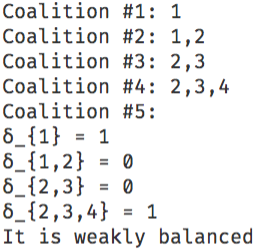
\includegraphics[scale=0.75]{console}
\end{figure}


\pagebreak
\section{The Bondareva-Shapley Theorem and Linear Programming}\label{sec:linearprogramming}
Finally, we will show that the Bondareva-Theorem holds true with a prove using the Duality Problem in Linear Programming.

\subsection{Introduction to Linear Programming}

\pagebreak

\vspace{-30pt}

\section*{Bonus: Minimal balanced collections for $N = 4$}\vspace{-6pt}\label{bonus}

\begin{tabular}{ | r l | c | }
    \multicolumn{2}{c}{Collection of coalitions} & \multicolumn{1}{c}{Coefficients}\\
    \hline & & \\[-10pt]
    $\mathcal{B}_{1} =$ & $\{\{1,2,3,4\}\}$ & $\left(1\right)$\\[2pt]
    $\mathcal{B}_{2} =$ & $\{\{2,3,4\}, \{1\}\}$ & $\left(1, 1\right)$\\[2pt]
    $\mathcal{B}_{3} =$ & $\{\{1,3,4\}, \{2\}\}$ & $\left(1, 1\right)$\\[2pt]
    $\mathcal{B}_{4} =$ & $\{\{1,2,4\}, \{3\}\}$ & $\left(1, 1\right)$\\[2pt]
    $\mathcal{B}_{5} =$ & $\{\{1,2,3\}, \{4\}\}$ & $\left(1, 1\right)$\\[2pt]
    $\mathcal{B}_{6} =$ & $\{\{3,4\}, \{1,2\}\}$ & $\left(1, 1\right)$\\[2pt]
    $\mathcal{B}_{7} =$ & $\{\{2,4\}, \{1,3\}\}$ & $\left(1, 1\right)$\\[2pt]
    $\mathcal{B}_{8} =$ & $\{\{2,3\}, \{1,4\}\}$ & $\left(1, 1\right)$\\[2pt]
    $\mathcal{B}_{9} =$ & $\{\{3,4\}, \{2\}, \{1\}\}$ & $\left(1, 1, 1\right)$\\[2pt]
    $\mathcal{B}_{10} =$ & $\{\{2,4\}, \{3\}, \{1\}\}$ & $\left(1, 1, 1\right)$\\[2pt]
    $\mathcal{B}_{11} =$ & $\{\{2,3\}, \{4\}, \{1\}\}$ & $\left(1, 1, 1\right)$\\[2pt]
    $\mathcal{B}_{12} =$ & $\{\{1,4\}, \{3\}, \{2\}\}$ & $\left(1, 1, 1\right)$\\[2pt]
    $\mathcal{B}_{13} =$ & $\{\{1,3\}, \{4\}, \{2\}\}$ & $\left(1, 1, 1\right)$\\[2pt]
    $\mathcal{B}_{14} =$ & $\{\{1,2\}, \{4\}, \{3\}\}$ & $\left(1, 1, 1\right)$\\[2pt]
    $\mathcal{B}_{15} =$ & $\{\{2,3,4\}, \{1,3,4\}, \{1,2\}\}$ & $\left(\frac{1}{2}, \frac{1}{2}, \frac{1}{2}\right)$\\[2pt]
    $\mathcal{B}_{16} =$ & $\{\{2,3,4\}, \{1,2,4\}, \{1,3\}\}$ & $\left(\frac{1}{2}, \frac{1}{2}, \frac{1}{2}\right)$\\[2pt]
    $\mathcal{B}_{17} =$ & $\{\{2,3,4\}, \{1,2,3\}, \{1,4\}\}$ & $\left(\frac{1}{2}, \frac{1}{2}, \frac{1}{2}\right)$\\[2pt]
    $\mathcal{B}_{18} =$ & $\{\{1,3,4\}, \{1,2,4\}, \{2,3\}\}$ & $\left(\frac{1}{2}, \frac{1}{2}, \frac{1}{2}\right)$\\[2pt]
    $\mathcal{B}_{19} =$ & $\{\{1,3,4\}, \{1,2,3\}, \{2,4\}\}$ & $\left(\frac{1}{2}, \frac{1}{2}, \frac{1}{2}\right)$\\[2pt]
    $\mathcal{B}_{20} =$ & $\{\{1,2,4\}, \{1,2,3\}, \{3,4\}\}$ & $\left(\frac{1}{2}, \frac{1}{2}, \frac{1}{2}\right)$\\[2pt]
    $\mathcal{B}_{21} =$ & $\{\{1\}, \{2\}, \{3\}, \{4\}\}$ & $\left(1, 1, 1, 1\right)$\\[2pt]
    $\mathcal{B}_{22} =$ & $\{\{1\}, \{2,3\}, \{2,4\}, \{3,4\}\}$ & $\left(1, \frac{1}{2}, \frac{1}{2}, \frac{1}{2}\right)$\\[2pt]
    $\mathcal{B}_{23} =$ & $\{\{1\}, \{2,3\}, \{2,4\}, \{1,3,4\}\}$ & $\left(\frac{1}{2}, \frac{1}{2}, \frac{1}{2}, \frac{1}{2}\right)$\\[2pt]
    $\mathcal{B}_{24} =$ & $\{\{1\}, \{2,3\}, \{3,4\}, \{1,2,4\}\}$ & $\left(\frac{1}{2}, \frac{1}{2}, \frac{1}{2}, \frac{1}{2}\right)$\\[2pt]
    $\mathcal{B}_{25} =$ & $\{\{1\}, \{2,4\}, \{3,4\}, \{1,2,3\}\}$ & $\left(\frac{1}{2}, \frac{1}{2}, \frac{1}{2}, \frac{1}{2}\right)$\\[2pt]
    $\mathcal{B}_{26} =$ & $\{\{2\}, \{1,3\}, \{1,4\}, \{3,4\}\}$ & $\left(1, \frac{1}{2}, \frac{1}{2}, \frac{1}{2}\right)$\\[2pt]
    $\mathcal{B}_{27} =$ & $\{\{2\}, \{1,3\}, \{1,4\}, \{2,3,4\}\}$ & $\left(\frac{1}{2}, \frac{1}{2}, \frac{1}{2}, \frac{1}{2}\right)$\\[2pt]
    $\mathcal{B}_{28} =$ & $\{\{2\}, \{1,3\}, \{3,4\}, \{1,2,4\}\}$ & $\left(\frac{1}{2}, \frac{1}{2}, \frac{1}{2}, \frac{1}{2}\right)$\\[2pt]
    $\mathcal{B}_{29} =$ & $\{\{2\}, \{1,4\}, \{3,4\}, \{1,2,3\}\}$ & $\left(\frac{1}{2}, \frac{1}{2}, \frac{1}{2}, \frac{1}{2}\right)$\\[2pt]
    $\mathcal{B}_{30} =$ & $\{\{3\}, \{1,2\}, \{1,4\}, \{2,4\}\}$ & $\left(1, \frac{1}{2}, \frac{1}{2}, \frac{1}{2}\right)$\\[2pt]
    $\mathcal{B}_{31} =$ & $\{\{3\}, \{1,2\}, \{1,4\}, \{2,3,4\}\}$ & $\left(\frac{1}{2}, \frac{1}{2}, \frac{1}{2}, \frac{1}{2}\right)$\\[2pt]
    $\mathcal{B}_{32} =$ & $\{\{3\}, \{1,2\}, \{2,4\}, \{1,3,4\}\}$ & $\left(\frac{1}{2}, \frac{1}{2}, \frac{1}{2}, \frac{1}{2}\right)$\\[2pt]
    $\mathcal{B}_{33} =$ & $\{\{3\}, \{1,4\}, \{2,4\}, \{1,2,3\}\}$ & $\left(\frac{1}{2}, \frac{1}{2}, \frac{1}{2}, \frac{1}{2}\right)$\\[2pt]
    $\mathcal{B}_{34} =$ & $\{\{4\}, \{1,2\}, \{1,3\}, \{2,3\}\}$ & $\left(1, \frac{1}{2}, \frac{1}{2}, \frac{1}{2}\right)$\\[2pt]
    $\mathcal{B}_{35} =$ & $\{\{4\}, \{1,2\}, \{1,3\}, \{2,3,4\}\}$ & $\left(\frac{1}{2}, \frac{1}{2}, \frac{1}{2}, \frac{1}{2}\right)$\\[2pt]
    $\mathcal{B}_{36} =$ & $\{\{4\}, \{1,2\}, \{2,3\}, \{1,3,4\}\}$ & $\left(\frac{1}{2}, \frac{1}{2}, \frac{1}{2}, \frac{1}{2}\right)$\\[2pt]
    $\mathcal{B}_{37} =$ & $\{\{4\}, \{1,3\}, \{2,3\}, \{1,2,4\}\}$ & $\left(\frac{1}{2}, \frac{1}{2}, \frac{1}{2}, \frac{1}{2}\right)$\\[2pt]
    $\mathcal{B}_{38} =$ & $\{\{1,2\}, \{1,3\}, \{1,4\}, \{2,3,4\}\}$ & $\left(\frac{1}{3}, \frac{1}{3}, \frac{1}{3}, \frac{2}{3}\right)$\\[2pt]
    $\mathcal{B}_{39} =$ & $\{\{1,2\}, \{2,3\}, \{2,4\}, \{1,3,4\}\}$ & $\left(\frac{1}{3}, \frac{1}{3}, \frac{1}{3}, \frac{2}{3}\right)$\\[2pt]
    $\mathcal{B}_{40} =$ & $\{\{1,3\}, \{2,3\}, \{3,4\}, \{1,2,4\}\}$ & $\left(\frac{1}{3}, \frac{1}{3}, \frac{1}{3}, \frac{2}{3}\right)$\\[2pt]
    $\mathcal{B}_{41} =$ & $\{\{1,4\}, \{2,4\}, \{3,4\}, \{1,2,3\}\}$ & $\left(\frac{1}{3}, \frac{1}{3}, \frac{1}{3}, \frac{2}{3}\right)$\\[2pt]
    $\mathcal{B}_{42} =$ & $\{\{1,2,3\}, \{1,2,4\}, \{1,3,4\}, \{2,3,4\}\}$ & $\left(\frac{1}{3}, \frac{1}{3}, \frac{1}{3}, \frac{1}{3}\right)$\\[2pt]
    \hline
\end{tabular}
 
\printbibliography
\end{document}